\documentclass{article}
\usepackage[letterpaper, margin = 1 in]{geometry}
\usepackage{graphicx}
\graphicspath{.}
\usepackage{float}

\begin{document}

\noindent \textbf{Flat Plate} \\ \\
Vortex of strength $\Gamma$ = -0.02 started upstream at (-4.5,0.04). Graph below shows comparison of obtained results to the analytical lift response of a flat plate to a passing vortex. Note that the lift for both analytical and numerical results have been `normalized' by the strength of the vortex $\Gamma$.\\
\begin{equation}
L = \rho \Gamma \frac{c}{2} e^{-kh} \big(-i S\big(k \big) \big)
\end{equation}

\begin{figure}[h]
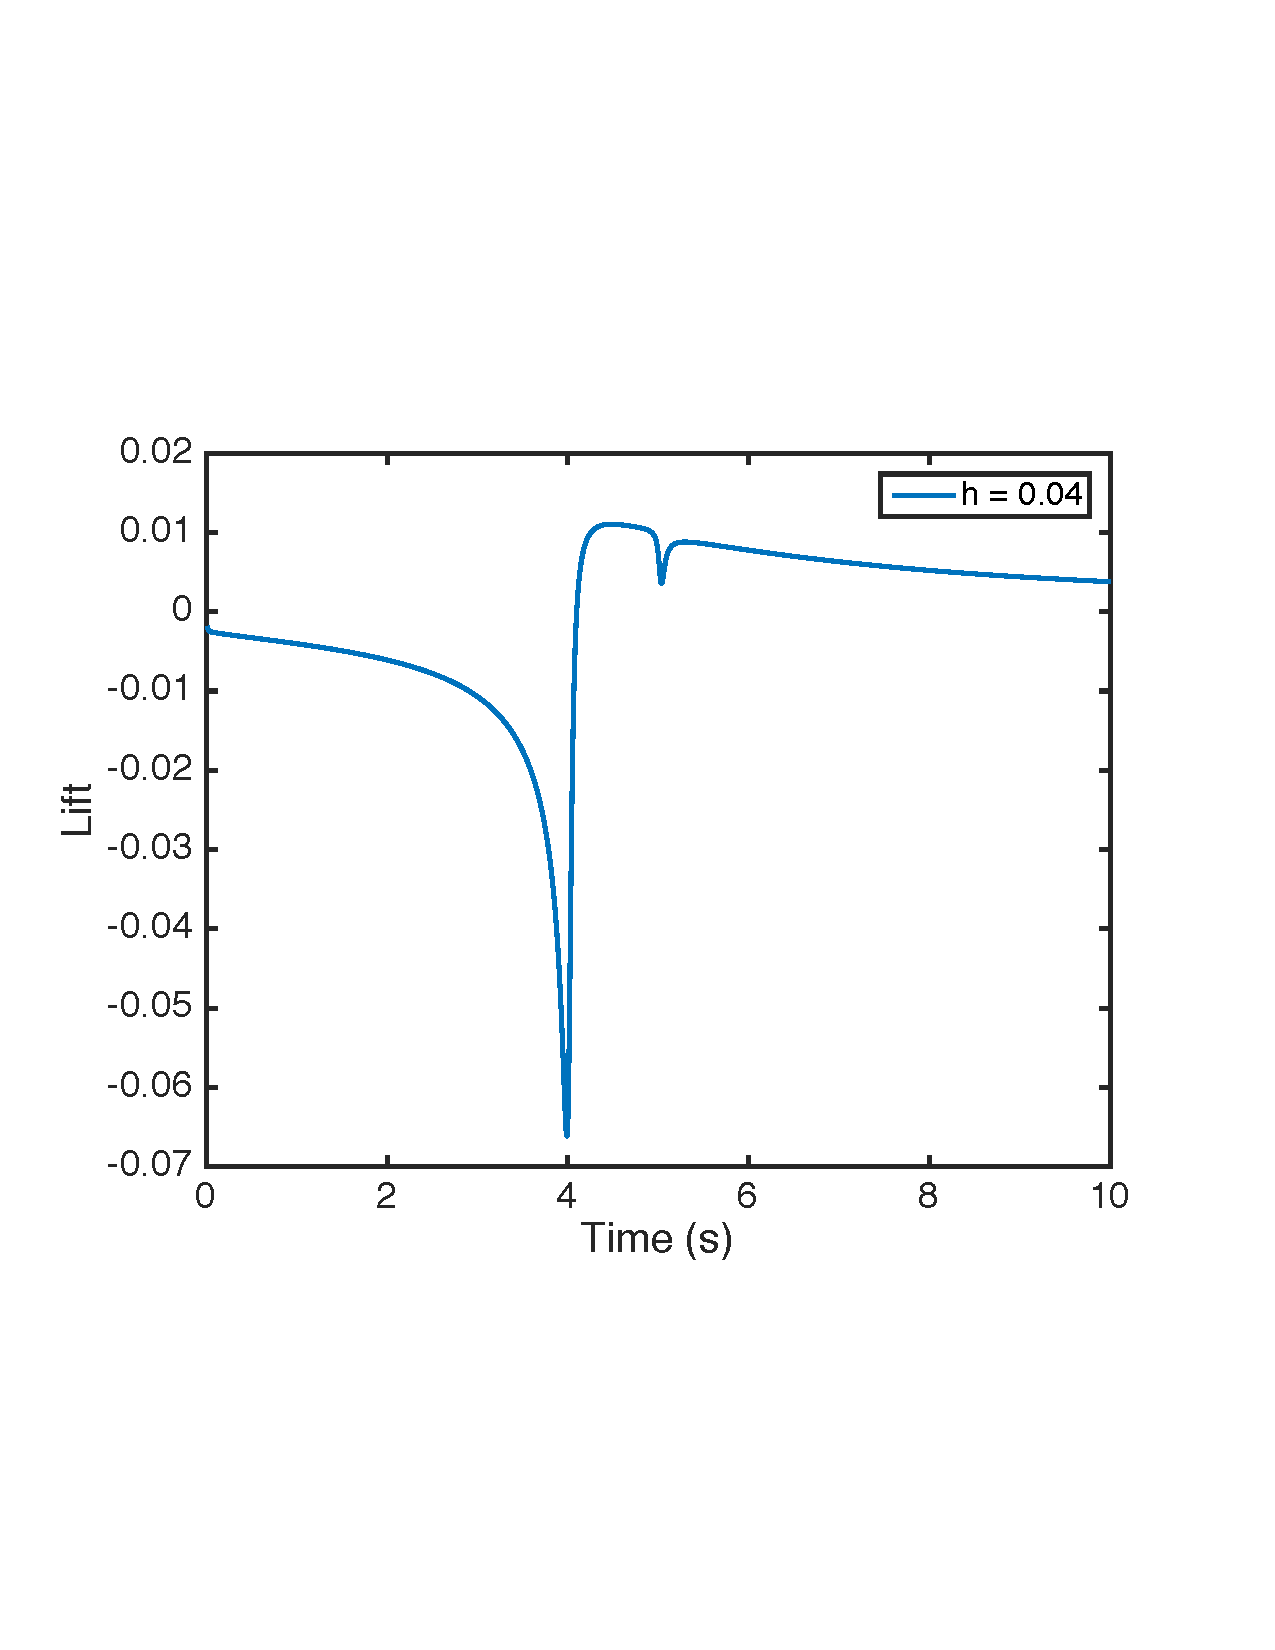
\includegraphics[width = 4 in, height = 3 in]{Lift_Curve}
\centering
\caption{Lift Curve Response of Flat Plate to Passing Vortex}
\end{figure}

\begin{figure}[h]
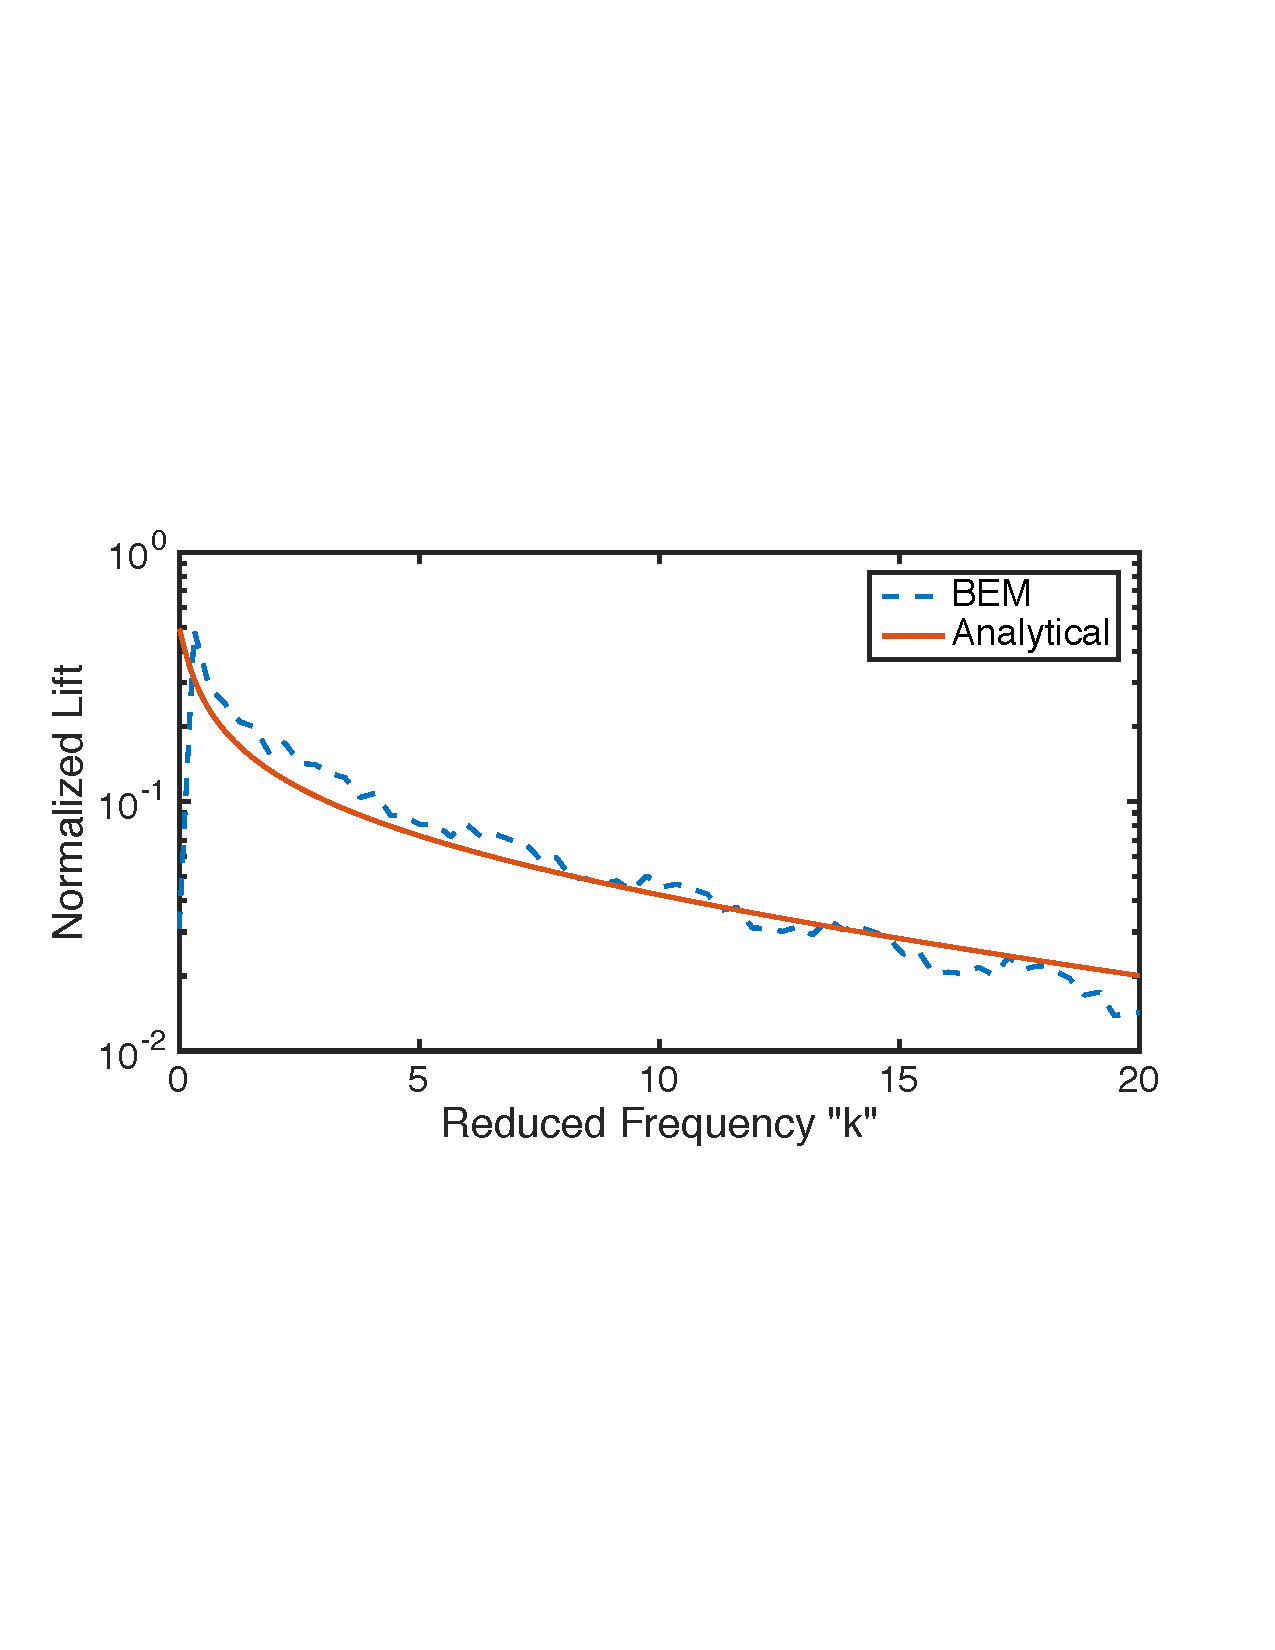
\includegraphics[width = 4 in, height = 3 in]{SearsVsBEM}
\centering
\caption{Analytical and BEM Spectrum of Lift for Vortex Passing Flat Plate}
\end{figure}
\newpage


\noindent For further validation purposes, the BVI results obtained from the Boundary Element method code was compared to other previously validated codes. The figure below shows the BEM results compared to Possio, an asymptotic method, and a method by Ayton. Also overlayed on the plot is the analytical Sears lift for the BVI problem. \\ \\
The asymptotic method, possio, and real AF method developed by Ayton are all gust problem approaches which require the user to input the mach numbers, angle of attack and spectral decompositions of the gust being studied. In the case of the BVI code, the height of passage of the imposed vortex becomes and important parameter. At higher frequencies, it is known that the lift scales as $exp(-kh)$ where h is the minimum passing distance of the vortex over the mean camber line of the airfoil. In order to obtain comparable results to the gust problem, this factor was removed from the obtained results and both lifts were appropriately normalized.

\begin{figure}[h]
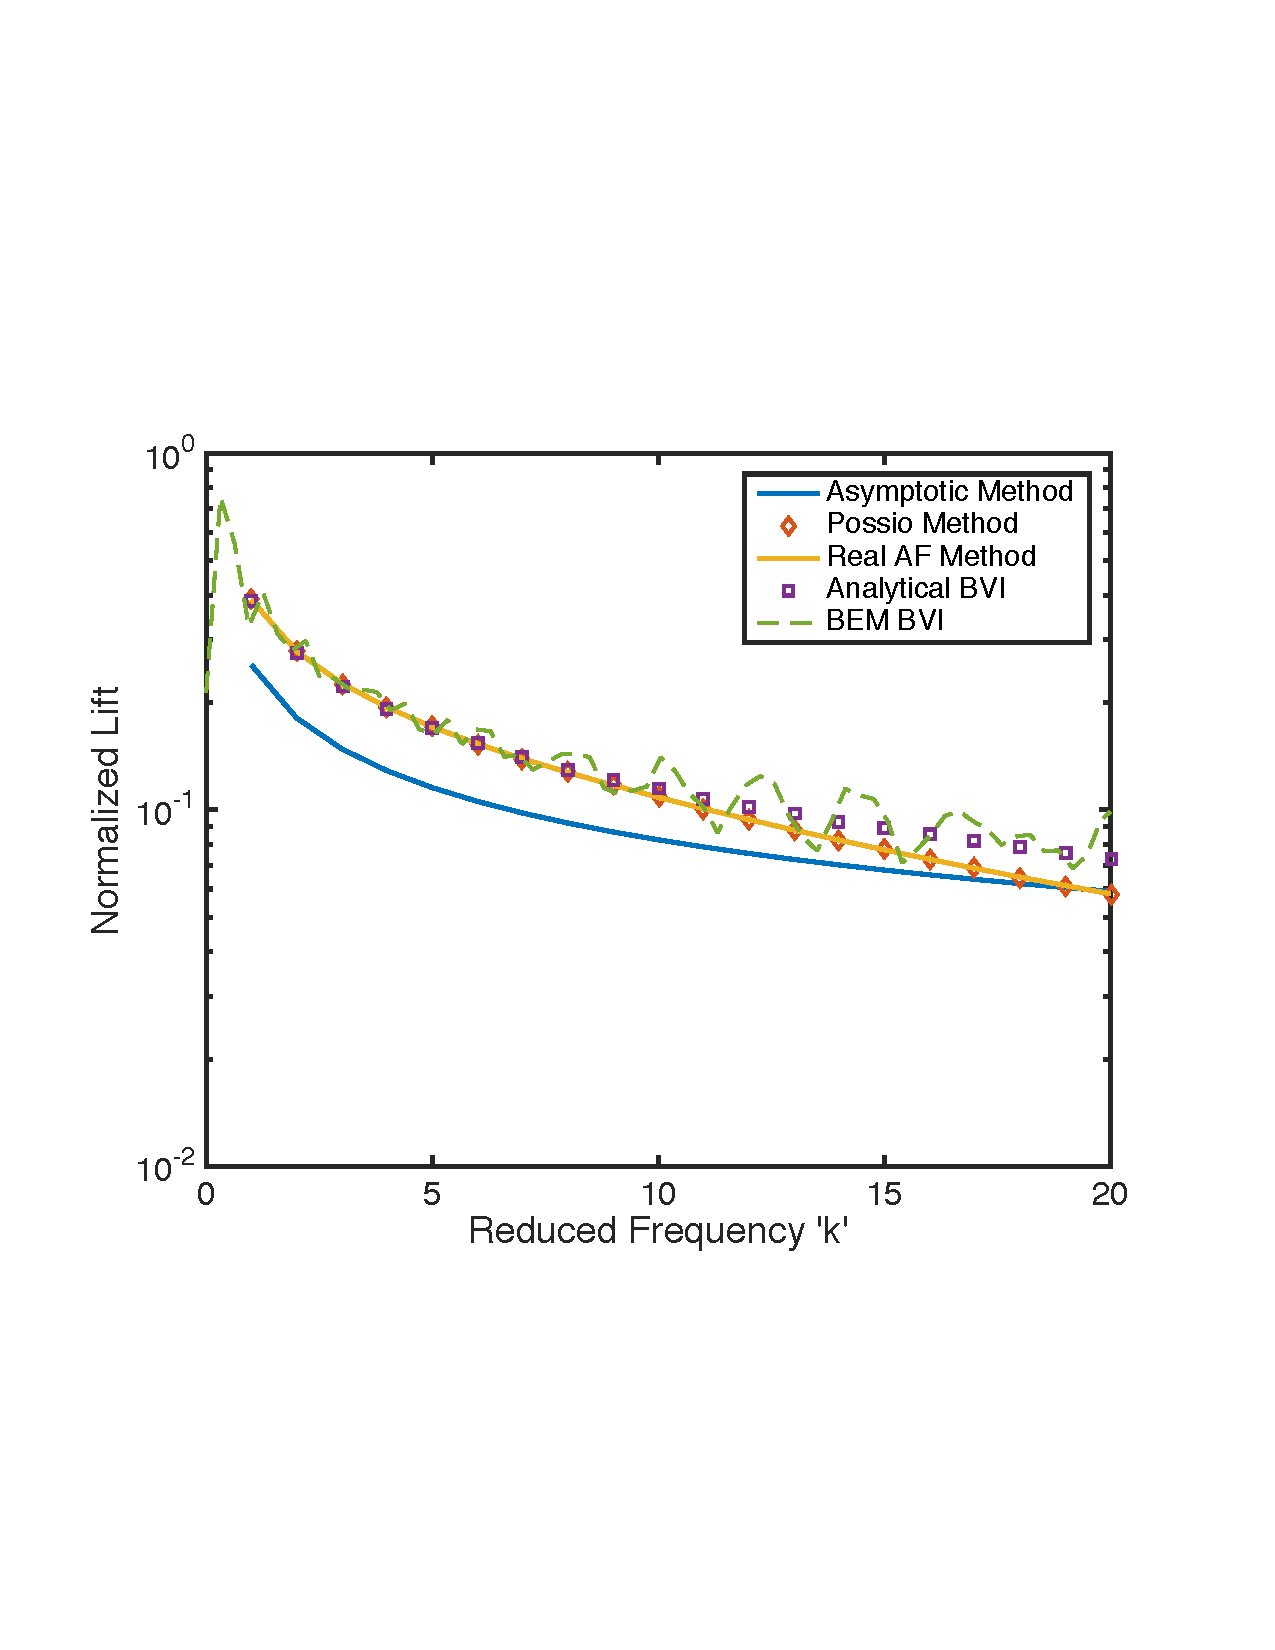
\includegraphics[width = 4 in, height = 3 in]{fp_total_compare}
\centering
\caption{Comparison of Lift Spectrums}
\end{figure}

\end{document}


